\chapter{Resultados}
\label{sec:resultados}

\section{Chat}
\label{sec:resultados:chat}

  \subsection{Objetivo}
    Esse chat foi com o intuito de ser uma prova de conceito do funcionamento da rede.
    Nele, um novo serviço chamado \textit{chat} seria adicionado, e a comunicação se daria
    através de mensagens anônimas enviadas a todos os nós conhecidos.
    
  \subsection{Implementação}
    O chat foi implementado utilizando o arcabouço \textit{LÖVE} para resolver o problema
    de como exibir uma nova mensagem enquanto pega entrada do usuário, assim como utilizar
    Lua para poder integrar com a implementação de exemplo do Etherclan.
    
    Referente às condições de uso do Etherclan, as seguintes escolhas foram realizadas:
    \begin{enumerate}
      \item Para bootstrap, temos um único IP/porta fixos no código.
      \item Como critério de quando realizar uma busca, elas são realizadas sempre que o
        usuário pressionar um botão.
      \item Como critério de quando remover um nó, eles nunca são removidos.
    \end{enumerate}
    
  \subsection{Resultado}
    \begin{figure}[h]
      \centering
      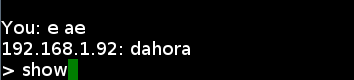
\includegraphics{../slides/chat.png}
      \caption{Parte visual do chat}
    \end{figure}
    
    Como prova de conceito, o chat foi um sucesso. Depois das buscas, mensagens são enviadas
    e recebidas com sucesso.
    
    Enquanto isso, na parte técnica, deixa muito a desejar. A \textit{LÖVE} não tem nenhuma
    forma decente de pegar texto bem formatado do usuário, incluindo acentuação e formatação.
    Fora isso, como as mensagens são enviadas de maneira síncrona utilizando TCP, cada nó
    inacessível acarreta em um atraso perceptível.
    
\section{Vikings Multijogador}
\label{sec:resultados:vikings}

  \subsection{Objetivo}
    Permitir que pelo menos dois jogadores se encontrem no mesmo mapa do \textit{vikings} e
    interajam em tempo real um com o outro. O processo de encontrar um outro jogador deve se
    passar inteiramente dentro do jogo, sem ter a necessidade de transferir informações como
    endereços.
    
  \subsection{Implementação}
    A busca de outros jogadores é realizada quando o jogador interage com um elemento do jogo,
    que então mostra uma lista de jogos acessíveis. Ao selecionar um jogo, é feito a transferência
    do mapa e de entidades do jogo, e então começa a sincronização de entrada com sincronização
    do estado de jogo periódicas.
    
    \begin{figure}[h]
      \centering
      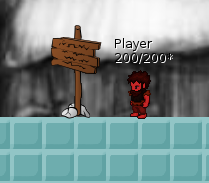
\includegraphics{imagens/vikings-signpost.png}
      \caption{Objeto de acesso às funções multi-jogador}
    \end{figure}
    
    \begin{figure}[h]
      \centering
      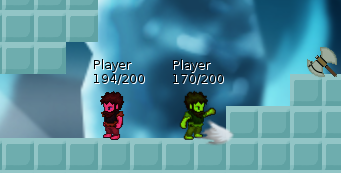
\includegraphics{imagens/vikings-multiplayer.png}
      \caption{Dois jogadores no mesmo mapa simultaneamente}
    \end{figure}

